%%
%% AAAI-27 Artificial Intelligence for Social Impact (AISI) Special Track
%% Anonymous submission. Built against the official AAAI-27 Author Kit
%% (aaai2027.sty / aaai2027.bst), copied alongside this file.
%%
\documentclass[letterpaper]{article}
\usepackage[submission]{aaai2027}
\usepackage[hyphens]{url}
\usepackage{graphicx}
\urlstyle{rm}
\def\UrlFont{\rm}
\usepackage{natbib}
\usepackage{caption}
\frenchspacing
\usepackage{booktabs}
\pdfinfo{
/TemplateVersion (2027.1)
}

\setcounter{secnumdepth}{1}

\title{Bridging the Data Gap: A Human-Validated Pipeline for\\
Culturally Aligned Topic Detection in Black Media}

\author{
    Anonymous Submission
}
\affiliations{
}

\begin{document}

\maketitle

\begin{abstract}
In the age of generative artificial intelligence, equitable AI development
requires training data that reflects the full breadth of human experience,
yet Black media publications remain systematically absent from major news
corpora such as C4 and Common Crawl. This absence embeds structural blind
spots into language models and limits their cultural alignment for Black
communities. We present a modular, open-source pipeline that continuously
scrapes, normalizes, and thematically annotates articles from ten prominent
Black media publications on a rolling monthly horizon, delivering
approximately 1,200 articles per cycle tagged against a curated taxonomy of
twelve social-conflict topics. To move beyond pipeline description, we
construct a 400-article human-annotated benchmark across two independent
annotators and conduct a rigorous comparative evaluation of six tagging
approaches: keyword matching, semantic similarity, three hybrid variants,
and a supervised classifier trained on sentence embeddings. We establish a
human agreement baseline through expert re-labeling and inter-annotator
agreement analysis, finding macro Cohen's kappa of 0.33 to 0.38, then show
that our best method, a per-topic logistic regression combining embeddings
with keyword and semantic signals, reaches 77 to 91 percent of that
baseline with a macro F1 of 0.322 and kappa of 0.297 under a leak-free
cross-annotator validation protocol. We release the pipeline code, taxonomy,
and annotation metadata to support replication and extension to other
under-represented media ecosystems. This work demonstrates that rigorous,
human-validated topic tagging of community media is achievable and offers a
transferable recipe for low-resource, equity-focused dataset infrastructure.
\end{abstract}

\section{Introduction}

Large language models are heavily shaped by their training data, and Black
media corpora are significantly absent from mainstream AI training
datasets, reflecting broader patterns of exclusion and misrepresentation in
AI data collection and model development \citep{bender2021}. Even with
non-profit web archives such as Common Crawl \citep{baack2024} providing
the raw material for datasets like C4, the Colossal Clean Crawled Corpus,
a filtered, cleaned web-text corpus used to pretrain the widely used T5
family of language models \citep{raffel2020}, there is currently no
widely recognized corpus explicitly curated as a Black media corpus;
instead, existing critiques indicate that downstream filtering can
exclude content associated with Black authors and other marginalized
groups \citep{baack2024}. This persistent
underrepresentation of Black media in foundational training corpora
contributes to the cultural misalignment increasingly observed in AI
systems, particularly in how these systems handle socially sensitive
issues affecting Black communities, where gaps in representation can
produce distorted, incomplete, or culturally insensitive responses
\citep{tao2024}.

The corpus-level absence described above is not only asserted in the
literature; we measure it directly. Auditing the Common Crawl snapshot
underlying C4, we find that nine of the ten Black media publications
monitored in this work have a combined footprint of fewer than 8,000 raw
captures, several orders of magnitude below single mainstream outlets such
as nytimes.com \citep{dodge2021}; the tenth, Capital B News, founded in
2022, cannot appear in the snapshot at all (Section~\ref{sec:gap}). We
monitor these ten publications through a continuously running collection
pipeline, an earlier version of which responded to this same absence by
building collection infrastructure for community media. But collection
alone leaves a critical question unanswered, one that reviewers of such
systems rightly press: are the produced topic labels reliable enough for
downstream research or model-development use? A pipeline that tags
articles with unvalidated heuristics produces a dataset whose labels
cannot be trusted, and an untrustworthy dataset serves the community it
documents poorly.

This paper answers that question for our pipeline, and in doing so offers
a template for answering it in other low-resource media ecosystems. We
make four contributions:

\begin{enumerate}
\item \textbf{An extended collection pipeline.} We expand coverage to ten
Black media publications, scraped on a rolling monthly horizon
($\sim$1{,}200 articles per cycle), tagged against a twelve-topic
social-conflict taxonomy, fully automated via CI/CD
(Section~\ref{sec:pipeline}).
\item \textbf{A human-annotated benchmark with an agreement baseline.} Two
independent annotators labeled 200 articles each; expert re-labeling of
all 400 yields inter-annotator agreement of macro $\kappa = 0.33$--$0.38$,
establishing the human baseline against which any automated tagger must
be read (Section~\ref{sec:annotation}).
\item \textbf{A leak-free comparative evaluation of six tagging methods.}
We compare keyword matching, semantic similarity, and hybrid variants
under cross-annotator validation, and document a threshold-tuning leak
whose correction reduces apparent performance by 0.07 macro F1
(Section~\ref{sec:eval}).
\item \textbf{A validated supervised classifier.} A per-topic logistic
regression over sentence embeddings, keyword, and semantic signals
reaches macro F1 0.322 and $\kappa$ 0.297, 77--91\% of the human baseline,
and is adopted as the pipeline's production tagger
(Sections~\ref{sec:methods}--\ref{sec:eval}).
\end{enumerate}

We frame this system as a foundational, incrementally validated pipeline
rather than a finished large-scale resource, and we prioritize
transparency about data sparsity and annotation difficulty over scale or
performance claims throughout (Section~\ref{sec:limitations}).

\section{Related Work}

\paragraph{Data equity and corpus documentation.}
A growing literature documents whose voices web-scale corpora contain.
\citet{dodge2021} audit C4 and show its domain distribution is dominated
by a small set of mainstream outlets; \citet{bender2021} argue that
undocumented, skewed corpora encode hegemonic viewpoints;
\citet{jo2020} draw on archival practice to propose deliberate,
consent-aware collection of sociocultural data; and \citet{gebru2021}
formalize dataset documentation itself. Disparities first quantified in
vision systems \citep{buolamwini2018} recur in text: under-representation
at the corpus level becomes mis-representation at the model level. Our
work operationalizes these critiques for one concrete ecosystem, the
Black press, by building and validating the missing data infrastructure.

\paragraph{Downstream bias measurement and mitigation.}
Corpus-level absence has measurable downstream consequences.
\citet{tao2024} evaluate cultural bias across large language models and
find that outputs skew toward dominant cultural values, while
\citet{an2025} document systematic racial bias in LLM-mediated decisions
such as automated resume screening. Reviews of this literature argue that
training data drawn mainly from majority populations produces weaker,
less reliable performance for marginalized groups, and recommend dataset
diversification, auditing, and human-centered design as mitigation
strategies \citep{kostickquenet2022,chen2023}. These studies motivate our
focus on label quality rather than collection scale alone: a pipeline
that is not validated against a human baseline cannot itself serve as
evidence that its data improves downstream alignment.

\paragraph{The Black press.}
The Black press has served as a parallel public sphere since Freedom's
Journal (1827), covering issues mainstream outlets ignored or distorted
\citep{washburn2006}. Its contemporary digital successors, from legacy
brands to digital natives founded in the last decade, are precisely the
outlets our audit shows to be absent from mainstream corpora, motivating
focused collection.

\paragraph{Topic detection and annotation quality.}
Topic assignment methods span keyword and seed-phrase matching,
embedding-based semantic similarity \citep{reimers2019}, and supervised
classification \citep{pedregosa2011}. Orthogonal to method choice is
label quality: chance-corrected agreement \citep{cohen1960} and its
interpretation \citep{landis1977,artstein2008} are standard in
computational linguistics but remain rare in dataset-infrastructure
papers, where system throughput is more commonly reported than label
validity. Our baseline agreement (macro $\kappa = 0.33$--$0.38$,
Section~\ref{sec:annotation}) falls within the fair-to-moderate range
\citet{landis1977} associate with subjective, low-prevalence
classification tasks, consistent with the difficulty such tasks are
known to pose for chance-corrected agreement more generally
\citep{artstein2008}. We treat agreement analysis as a first-class
component of the pipeline.

\section{Pipeline Overview}
\label{sec:pipeline}

The pipeline (Figure~\ref{fig:pipeline}) runs monthly via GitHub Actions
and comprises four stages. \textbf{Scrape:} source-specific scrapers
(WordPress REST, HTML, RSS fallback) collect every article published by
ten Black media publications within a rolling window matching the
calendar month, yielding $\sim$1{,}200 articles per cycle. \textbf{Analyze:}
each article (title, description, and body text) is tagged against the
twelve-topic social-conflict taxonomy of Table~\ref{tab:taxonomy} by the
production tagger (the supervised classifier validated in this paper).
\textbf{Report:} the run exports research-ready CSV artifacts and a
styled PDF editorial summary. \textbf{Deliver:} artifacts are deposited
to a shared cloud drive for non-technical stakeholders.

\begin{figure}[t]
\centering
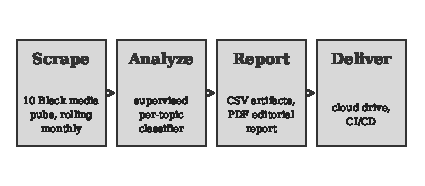
\includegraphics[width=0.9\columnwidth]{figures/fig_pipeline.pdf}
\caption{The four-stage pipeline. This paper's contribution is the
validation of the \emph{Analyze} stage: the supervised classifier adopted
there is the best of six methods evaluated against a 400-article human
benchmark.}
\label{fig:pipeline}
\end{figure}

The taxonomy was curated with domain collaborators to cover the
social-conflict issues most consistently central to Black media coverage.
Articles may carry multiple topics or none; in practice a large share of
the feed (sports, entertainment, lifestyle) falls outside the taxonomy
entirely, which has direct consequences for annotation
(Section~\ref{sec:annotation}).

\begin{table}[t]
\centering
\small
\begin{tabular}{lrr}
\toprule
& \multicolumn{2}{c}{Human positives} \\
\cmidrule(lr){2-3}
Topic & Set 1 & Set 3 \\
\midrule
Policing / Public Safety        & 23 & 13 \\
Economic Equity / Wealth Gap    & 47 & 30 \\
Housing / Displacement          & 14 &  9 \\
Environmental Justice           & 14 &  7 \\
Voter Suppression               & 13 &  3 \\
Criminal Justice Reform         &  7 &  8 \\
School Funding                  &  7 &  3 \\
Redlining / Fair Housing        &  5 &  0 \\
Reparations                     &  5 &  0 \\
Book Bans / Anti-DEI            &  4 &  4 \\
Maternal Health                 &  4 &  4 \\
Anti-Black Surveillance         &  3 &  0 \\
\midrule
Total label decisions           & \multicolumn{2}{c}{$400 \times 12 = 4{,}800$} \\
\bottomrule
\end{tabular}
\caption{The twelve-topic social-conflict taxonomy with the number of
positive human labels in each 200-article annotation set. The long tail
is severe: three topics have zero positives in Set 3, a sparsity that
shapes every result in this paper.}
\label{tab:taxonomy}
\end{table}

\section{Measuring the Data Gap}
\label{sec:gap}

Earlier presentations of this pipeline asserted that its sources are
missing from mainstream corpora; here we measure it. C4
\citep{raffel2020} was filtered from the Common Crawl snapshot
CC-MAIN-2019-18. We queried the Common Crawl index for every capture of
each of our ten publication domains in that snapshot
(Table~\ref{tab:audit}). Because C4's filters (English-only,
deduplication, blocklists, length heuristics) only \emph{remove} pages,
these counts upper-bound each domain's possible C4 presence.

\begin{table}[t]
\centering
\small
\begin{tabular}{lr}
\toprule
Domain & Captures in CC-MAIN-2019-18 \\
\midrule
blavity.com        & 3{,}774 \\
theroot.com        & 1{,}291 \\
ebony.com          &   911 \\
thegrio.com        &   881 \\
essence.com        &   407 \\
newsone.com        &   203 \\
afrotech.com       &   186 \\
21ninety.com       &   113 \\
capitalbnews.org   &     0 \\
travelnoire.com    &   n/a\textsuperscript{*} \\
\midrule
Combined (measured) & 7{,}766 \\
\bottomrule
\end{tabular}
\caption{Presence of our ten publication domains in the Common Crawl
snapshot from which C4 was built. \textsuperscript{*}Index query
unresolved at submission time. For scale, \emph{nytimes.com} is among
the largest domains in all of C4 \citep{dodge2021}.
\emph{Capital B News} (founded 2022) post-dates the snapshot entirely.}
\label{tab:audit}
\end{table}

The combined measured footprint of nine of our ten domains, 7,766 raw
captures before C4's aggressive filtering, is several orders of magnitude
smaller than that of a single mainstream outlet. The \emph{Capital B}
result generalizes: any publication founded after a corpus's snapshot
date is structurally invisible to models trained on it, and community
media skews young. Continuous collection, not one-time archival, is
therefore the appropriate remedy, which is what the pipeline provides.

\section{Human Annotation and Agreement}
\label{sec:annotation}

\paragraph{Protocol.}
Two independent annotators each labeled a disjoint set of 200 articles
sampled from a pipeline run, marking, for each article, every applicable
topic among the twelve (binary decisions; multi-label; no topic is also
valid). This yields $4{,}800$ label decisions. To measure agreement, a
domain expert on the research team independently re-labeled all 400
articles under the same guidelines.

\paragraph{Results.}
Figure~\ref{fig:iaa} reports per-topic Cohen's $\kappa$ \citep{cohen1960}
between the expert and each original annotator. Macro-averaged over
topics, agreement is $\kappa = 0.327$ against Annotator~1 and
$\kappa = 0.384$ against Annotator~3; pooled over all decisions,
$\kappa = 0.410$ and $0.531$ respectively, fair-to-moderate on
conventional scales \citep{landis1977}.

\begin{figure}[t]
\centering
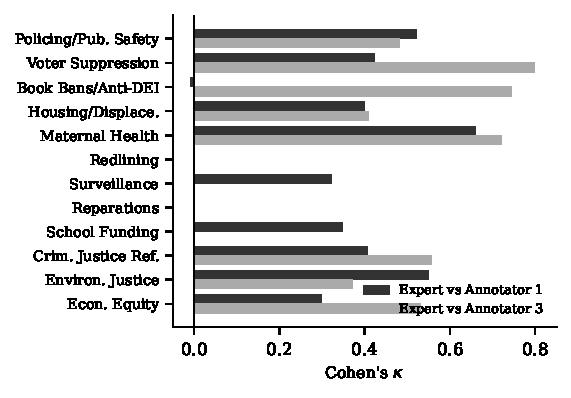
\includegraphics[width=0.9\columnwidth]{figures/fig_iaa.pdf}
\caption{Per-topic inter-annotator agreement (Cohen's $\kappa$) between
the expert re-labeling and each original annotator. Zero bars are topics
with no positive labels from either party; agreement there is undefined
in practice.}
\label{fig:iaa}
\end{figure}

\paragraph{Why agreement is moderate, and why we report it anyway.}
We treat the manual annotation as a \emph{baseline standard, not perfect
ground truth}, and the $\kappa$ values as a finding about the task
rather than a defect of the study. Three factors depress agreement, all
visible in Table~\ref{tab:taxonomy} and Figure~\ref{fig:iaa}. First,
\emph{topic sparsity}: five topics have five or fewer positives per set,
and three have none at all in Set~3; with so few positives, a single
disagreement swings $\kappa$ dramatically, and $\kappa$ is undefined or
uninformative at zero prevalence \citep{artstein2008}. Second,
\emph{feed composition}: much of the scraped stream is sports,
entertainment, and lifestyle coverage outside the taxonomy, so
annotators spend most decisions confirming absence, and the rare
positive cases concentrate the ambiguity. Third, \emph{boundary
overlap}: the hardest topics are those with genuinely contested
boundaries: \emph{Economic Equity} absorbs stories that also touch
housing or schooling, and platform-side miscategorization (e.g.,
policing stories filed under generic ``politics'') seeds anchoring
disagreements. An automated tagger evaluated against labels of this
character cannot meaningfully exceed them; it can only approach them.
That is the yardstick we adopt.

\section{Tagging Methods}
\label{sec:methods}

We evaluate six methods, in increasing order of supervision.

\paragraph{Keyword tagger.}
Curated seed phrases per topic, matched against title, description, and
body. High precision on explicit mentions; blind to paraphrase.

\paragraph{Semantic tagger.}
Cosine similarity between the article embedding and per-topic seed-text
embeddings, using \texttt{all-MiniLM-L6-v2} \citep{reimers2019}, with a
global decision threshold. Recovers paraphrase; noisier near the
threshold.

\paragraph{Hybrid OR / AND.}
Union and intersection of the two base taggers' positive sets. OR
maximizes recall at heavy precision cost; AND the reverse.

\paragraph{Hybrid Soft Boost.}
Keyword matches always fire; additionally, the semantic score can fire a
topic if it clears a \emph{per-topic} threshold grid-searched to maximize
F1. We evaluate this in two forms. The \emph{in-sample} form tunes
thresholds on the same annotator set used for scoring; this is the
version with a tuning leak, retained deliberately as an upper bound and
as a documented cautionary result. The \emph{cross-validated (CV)} form
tunes thresholds on one annotator's 200 articles and applies them to the
other's, eliminating the leak.

\paragraph{Supervised classifier.}
One logistic regression per topic \citep{pedregosa2011}, with
class-balanced weighting, over a feature vector concatenating (i)~the
384-dimensional sentence embedding of the article text, (ii)~the keyword
tagger's binary decision, and (iii)~the raw semantic score for that
topic. Training and testing follow the same cross-annotator protocol as
Soft Boost (CV): train on Annotator~1's set, test on Annotator~3's, and
vice versa. Topics with fewer than two positive training examples fall
back to the keyword decision; this occurred for three topics in one
direction (Redlining, Surveillance, and Reparations, namely the zero-
prevalence topics of Table~\ref{tab:taxonomy}) and is flagged in all
reported results.

\section{Evaluation}
\label{sec:eval}

\paragraph{Protocol.}
All methods are scored against both annotator sets on per-topic
precision, recall, F1, and Cohen's $\kappa$, macro-averaged over the
twelve topics and pooled across the two sets. Methods requiring tuning
or training never see the set they are scored on: this cross-annotator
validation is a deliberately harsh test, since the annotators themselves
agree only at $\kappa = 0.33$--$0.38$, so any tuned artifact must survive
both sampling variance and genuine annotator shift.

\paragraph{The threshold-tuning leak.}
Table~\ref{tab:results} reports Soft Boost both ways. In-sample tuning
yields macro F1 0.336; the leak-free CV form yields 0.267. The 0.07 gap
(21\% of the apparent score) was pure tuning optimism, and the honest
hybrid is statistically indistinguishable from the untuned semantic
baseline (0.266). We highlight this because per-topic threshold tuning
on evaluation data is common, tempting, and in low-prevalence regimes
like ours, badly misleading.

\begin{table}[t]
\centering
\small
\begin{tabular}{lcc}
\toprule
Method & Macro F1 & Macro $\kappa$ \\
\midrule
Keyword                    & 0.214 & 0.183 \\
Semantic                   & 0.266 & 0.225 \\
Hybrid OR                  & 0.229 & 0.181 \\
Hybrid AND                 & 0.259 & 0.244 \\
Hybrid Soft Boost (in-sample)\textsuperscript{\dag} & 0.336 & 0.297 \\
Hybrid Soft Boost (CV)     & 0.267 & 0.224 \\
\textbf{Supervised (CV)}   & \textbf{0.322} & \textbf{0.297} \\
\midrule
Human baseline (IAA)       & n/a & 0.327--0.384 \\
\bottomrule
\end{tabular}
\caption{Pooled macro-averaged results over both annotator sets.
\textsuperscript{\dag}In-sample Soft Boost tunes thresholds on the
evaluation data and is reported only as an upper bound; all other tuned
or trained methods use leak-free cross-annotator validation. The
supervised classifier is the best honest method and matches the leaked
upper bound's $\kappa$.}
\label{tab:results}
\end{table}

\paragraph{Main result.}
The supervised classifier attains macro F1 0.322 and $\kappa$ 0.297
under the leak-free protocol (Figure~\ref{fig:methods}), a 21\% relative
F1 improvement over the best honest alternative, and a $\kappa$ equal to
the \emph{leaked} Soft Boost upper bound. Measured against the human
agreement baseline, the classifier reaches 91\% of the Set~1 ceiling
($0.297/0.327$) and 77\% of the Set~3 ceiling ($0.297/0.384$). Both
cross-annotator directions agree closely (F1 0.326 testing on Set~3;
0.319 testing on Set~1), indicating the result is not an artifact of one
annotator's style.

\paragraph{Statistical significance.}
With 200 test articles per direction and the sparsity documented in
Table~\ref{tab:taxonomy}, the gap between the supervised classifier and
the best honest hybrid (Soft Boost CV) could plausibly be sampling noise
rather than a real effect. We test this with a paired bootstrap:
resampling the test articles with replacement (5{,}000 resamples per
direction, both methods scored on the identical resampled articles each
iteration) and recomputing the pooled macro F1 and $\kappa$ gap every
time. The F1 gap (+0.055) is positive in 98.5\% of resamples (95\% CI
$[0.005, 0.099]$, two-sided $p = 0.030$); the $\kappa$ gap (+0.073) is
positive in 99.8\% of resamples (95\% CI $[0.021, 0.118]$, two-sided
$p = 0.005$). The supervised classifier's advantage is therefore unlikely
to be a resampling artifact, though the F1 gap's interval sits close to
zero and should be read as a modest, not decisive, margin.

\begin{figure*}[t]
\centering
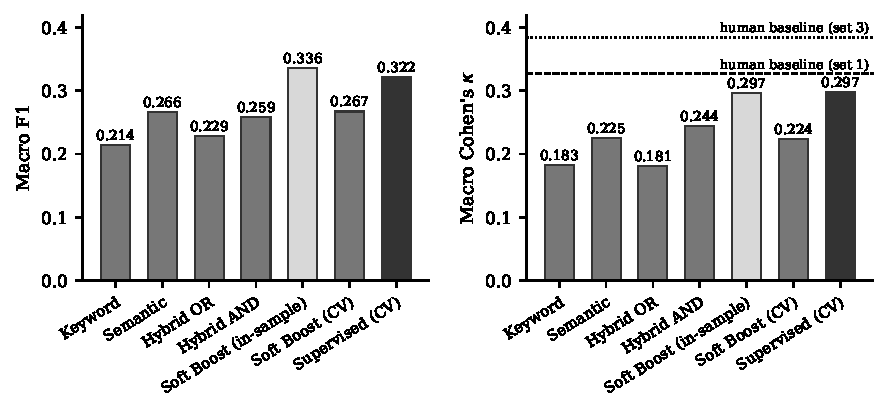
\includegraphics[width=0.8\textwidth]{figures/fig_methods.pdf}
\caption{Macro F1 (left) and Cohen's $\kappa$ (right) for all methods.
Dashed and dotted lines mark the human agreement baselines from the IAA
study. The supervised classifier (dark) is the only honest method whose
$\kappa$ approaches the human range; the in-sample Soft Boost bar (pale)
is the documented leaked upper bound.}
\label{fig:methods}
\end{figure*}

\paragraph{Per-topic behavior.}
Figure~\ref{fig:pertopic} breaks the supervised result down by topic and
direction. Performance tracks prevalence: the well-populated topics
(Economic Equity, Policing, Housing, Criminal Justice Reform,
Environmental Justice) reach F1 0.42--0.62, while the zero- and
near-zero prevalence topics (Redlining, Reparations, Surveillance) are
unmeasurable: no method can be evaluated on topics for which humans
found no positive examples. We report these as unmeasurable rather than
as zeros of model quality; expanding annotation for rare topics is
future work, not a solved problem.

\begin{figure}[t]
\centering
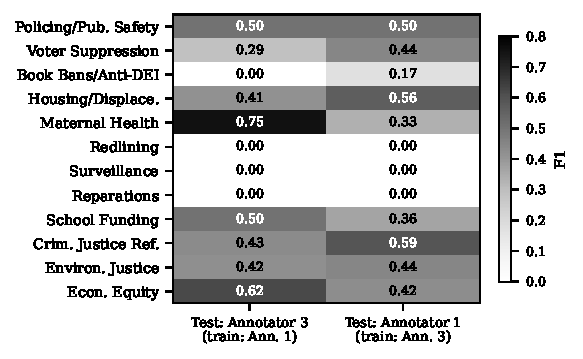
\includegraphics[width=0.9\columnwidth]{figures/fig_pertopic.pdf}
\caption{Per-topic supervised F1 in both cross-annotator directions.
Performance concentrates where human labels exist (cf.\
Table~\ref{tab:taxonomy}); blank-prevalence topics are unmeasurable.}
\label{fig:pertopic}
\end{figure}

\paragraph{Production adoption.}
On these results the supervised classifier, retrained on all 400 labeled
articles, replaces the keyword matcher as the pipeline's production
tagger. The frozen 400-article benchmark and evaluation scripts run in
CI, so future modifications to the tagger or taxonomy are automatically
scored against the human baseline before deployment.

\section{Limitations}
\label{sec:limitations}

\paragraph{Moderate agreement, honestly reported.}
Our human baseline ($\kappa$ 0.33--0.38 macro) is fair-to-moderate, and
we have argued this reflects task structure (sparsity, feed composition,
boundary overlap) rather than careless annotation. Nonetheless, all
downstream numbers inherit this uncertainty, and readers should treat
per-topic scores on sparse topics as indicative at best.

\paragraph{Anchoring risk.}
Original annotation sheets displayed the keyword pipeline's predictions,
which may anchor annotators toward them; the expert re-labeling was
performed blind to predictions, but the original labels were not.

\paragraph{Two annotators, one expert.}
The IAA study spans two annotator-expert pairs; a larger annotator pool
would tighten the baseline estimate.

\paragraph{No downstream experiment yet.}
We validate label quality, not downstream impact on model behavior;
demonstrating that this data measurably improves cultural alignment of a
language model is the natural next study, enabled but not performed by
this work.

\section{Discussion and Future Work}
\label{sec:discussion}

We frame this system as a foundational, incrementally validated pipeline
rather than a finished large-scale resource. The core result, a
supervised classifier reaching 77--91\% of a human-agreement ceiling
that is itself only fair-to-moderate, should be read in that light: it
says the tagger is about as good as it can be given labels of this
character, not that either the labels or the tagger are done improving.

\paragraph{Scale versus validity.}
Restricting collection to articles plainly within the twelve topics
would raise every metric in this paper, at the cost of a smaller, less
representative resource. For this submission we kept the full-feed scale
and reported the resulting sparsity transparently; stricter subtopic
filtering is a tunable choice we leave to dataset users rather than a
decision we make for them.

These two limitations point directly at what comes next. Broader
annotation for rare topics (Redlining, Reparations, Anti-Black
Surveillance) would resolve the unmeasurable cells in
Figure~\ref{fig:pertopic} and let the taxonomy's long tail be evaluated
rather than assumed. A larger, more diverse annotator pool would tighten
the IAA baseline itself, which is currently the ceiling every other
number in the paper is measured against. Extending the pipeline to
additional community media ecosystems beyond the Black press would test
whether this recipe generalizes. And the downstream experiment we have
not yet run, measuring whether training or fine-tuning on this data
measurably improves a language model's cultural alignment, is the
natural next study this infrastructure now enables.

\section{Conclusion}

We presented a continuously running pipeline for collecting and
thematically tagging Black media coverage. Its core contribution is a
human-validated evaluation of the tagging stage: a measured corpus audit
grounds the motivating data gap; a 400-article benchmark with expert
re-labeling establishes a human agreement baseline; a documented
threshold-tuning leak and its correction establish honest evaluation
practice; and a supervised classifier reaching 77--91\% of the human
baseline becomes the production tagger. Code, taxonomy, evaluation
scripts, and annotation metadata (URLs, labels, and scores; not full
article text, respecting publisher copyright) will be released upon
publication.

\bibliography{aisi2027}

\end{document}
